\chapter{Definitions}

\section{Module}
One module in Plantage is just a rectangular shape. From that point of view every circuit element can be seen as modules, transistors, capacitors and so on. For the placement only width and height of the module are important. The actual dimensions are stored in the variant of the module. Every module can have various different variants, for example, with the same electrical behaviour, but different numbers of gates \nref{fig:modules_with_different_gate_number}.

\begin{figure}
	\centering
	\setlength{\unitlength}{0.282222229121mm}
\begin{picture}(520.0, 200.0)(0, -200.0)
  \put(0,-200.0){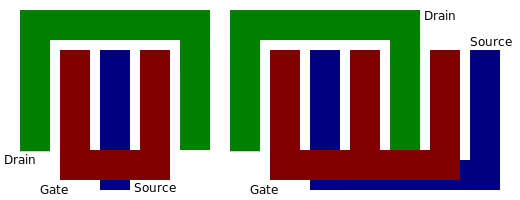
\includegraphics[height=56.4444458242mm, width=146.755559143mm]{FIG/modules_with_different_gate_number.svg.pdf}}
  \put(40.0,-194.00002){\makebox(0,0)[l]{\smash{Gate}}}
  \put(4.0,-164.00002){\makebox(0,0)[l]{\smash{Drain}}}
  \put(134.0,-192.00002){\makebox(0,0)[l]{\smash{Source}}}
  \put(250.0,-194.00002){\makebox(0,0)[l]{\smash{Gate}}}
  \put(424.0,-20.0){\makebox(0,0)[l]{\smash{Drain}}}
  \put(470.0,-46.0){\makebox(0,0)[l]{\smash{Source}}}
\end{picture}
	\caption{the same MOSFET with two different numbers of gates}
	\label{fig:modules_with_different_gate_number}
\end{figure}

Also a module typically has some pins, which are named and, additionally, have a net name as well, according to the net they belong to. One pin can have some contact areas, but must have at least one. Every contact area is only a rectangular shape, which has a height and width and is in a relative position to the module position.

\section{Group}
In Plantage there are two different types of groups. One type contains only groups and the other one only modules \nref{fig:group_of_modules}. At the moment it is not possible to mix modules and groups in one group. This is important because slightly different algorithms must be applied for every type of group.

\begin{figure}
	\centering
	\subfloat[group of single modules]{
\includegraphics[scale=0.5]{FIG/group_of_modules.png}}
	\subfloat[group of two groups]{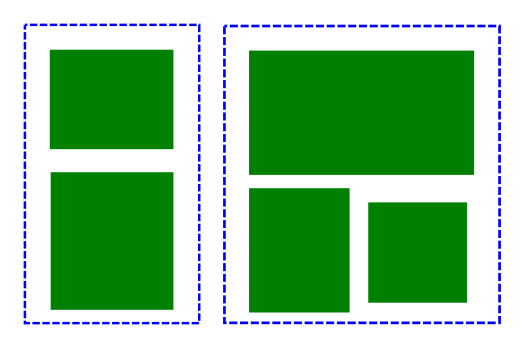
\includegraphics[scale=0.5]{FIG/group_of_groups.png}}
	\caption{groups arrange modules and groups together}
	\label{fig:group_of_modules}
\end{figure}

\section{Shape Function}
A shape function is basically a list of possible layouts for a given circuit. This list is called shape function \nref{fig:shapefunction} because the minimum possible area for these placements is a hyperbolic function and the placements are located near this so-called \emph{pareto front}.

\begin{figure}
	\centering
	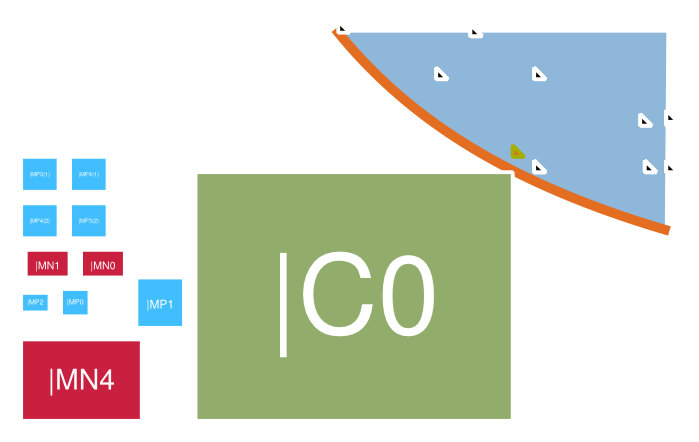
\includegraphics[scale=1.8]{FIG/shapefunction.png}
	\caption{shapefunction with possible placements for a miller amplifier}
	\label{fig:shapefunction}
\end{figure}

\subsection{Shape}
A shape is the layout for a certain couple of modules. On the one hand, it is used for the layout of the whole circuit but, on the other hand, also for the layout of circuit parts.

\section{Constraints}
In the design of analog circuits many constraints have to be met. They mainly consider that certain elements of the circuit should have similar electrical characteristics as far as possible. The most prominent example for such a pair of modules are the parts of a differential pair. Differences in these transistors result in a bigger offset of the resulting amplifier, which should be as low as possible.

\subsection{Symmetry Constraint}
\label{subsec:symmetry_constraint}
Symmetry constraints define a vertical or horizontal symmetry axis for modules. They can contain two different types: single modules and pair modules. Single modules are placed self-symmetrically to the axis, pair modules are symmetric pairwise. For the symmetry only the centers of gravity are considered, therefore pair modules can have different shapes. \nref{fig:constraint_symmetry}

\begin{figure}
	\centering
	\setlength{\unitlength}{0.282222229121mm}
\begin{picture}(400.0, 300.0)(0, -300.0)
  \put(0,-300.0){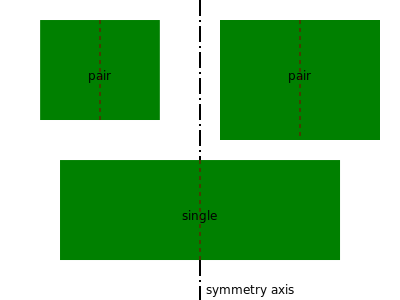
\includegraphics[height=84.6666687363mm, width=112.888891648mm]{FIG/constraint_symmetry.svg.pdf}}
  \put(206.0,-294.00002){\makebox(0,0)[l]{\smash{symmetry axis}}}
  \put(88.0,-80.0){\makebox(0,0)[l]{\smash{pair}}}
  \put(288.0,-80.0){\makebox(0,0)[l]{\smash{pair}}}
  \put(182.0,-220.0){\makebox(0,0)[l]{\smash{single}}}
\end{picture}
	\caption{horizontal symmetry constraint with one pair of modules and one single module}
	\label{fig:constraint_symmetry}
\end{figure}

\subsection{Alignment Constraint}
An alignment constraint defines a relative position between modules, vertical or horizontal \nref{fig:constraint_alignment}. In the terminology of Plantage you always have a A- and a B-module. In the case of a horizontal alignment the A-module is placed left to the B-module, in the other case of a vertical alignment the A-module is placed below the B-module. Additionally, it is possible to define a minimum distance between the modules.

\begin{figure}
	\centering
	\setlength{\unitlength}{0.282222229121mm}
\begin{picture}(400.0, 200.0)(0, -200.0)
  \put(0,-200.0){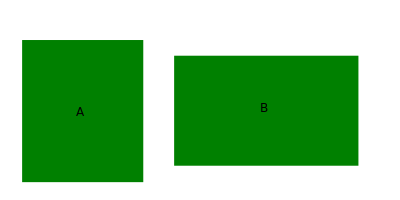
\includegraphics[height=56.4444458242mm, width=112.888891648mm]{FIG/constraint_alignment.svg.pdf}}
  \put(76.0,-116.0){\makebox(0,0)[l]{\smash{A}}}
  \put(260.0,-112.0){\makebox(0,0)[l]{\smash{B}}}
\end{picture}
	\caption{horizontal alignment constraint}
	\label{fig:constraint_alignment}
\end{figure}

\subsection{Group Symmetry Constraint}
The group symmetry constraint is nearly the same as the symmetry constraint. The only difference is that it can be applied to groups instead of modules. Like the normal symmetry constraint we can have single groups, which are self-symmetrically placed, or pair groups, which are pairwise symmetric to the symmetry axis.

\subsection{Group Alignment Constraint}
Once again the group alignment constraint is nearly the same as the alignment constraint where the only difference is that it can be applied to groups.

\subsection{Same Variants Constraint}
The same variants constraint is very important too, for example, especially for differential pairs. To get the same characteristics in one placement as far as possible these modules should have the same variants. They can still have various different variants, but in one certain placement for these modules the same variant is selected.

The implementation of this constraint is based on matching the names of the variants. Therefore it is still possible that the variants differ, for example the variant for one module is mirrored to the ones of the other part of a pair. This is very useful, as it gives the user a lot more flexibility.

\section{Technology Rules}

\begin{figure}
	\centering
	\setlength{\unitlength}{0.282222229121mm}
\begin{picture}(400.0, 200.0)(0, -200.0)
  \put(0,-200.0){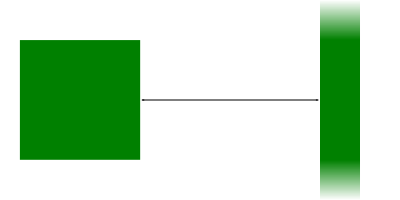
\includegraphics[height=56.4444458242mm, width=112.888891648mm]{FIG/technology_rule_spacing.svg.pdf}}
  \put(176.0,-94.0){\makebox(0,0)[l]{\smash{minimum spacing}}}
\end{picture}
	\caption{minimum spacing rule}
	\label{fig:technology_rule_spacing}
\end{figure}

Typically, the manufacturer of the chip provides a so-called \textit{tech-file} for the circuit designer, which can be used to create the layout. This information includes, for example, the minimum distances between two modules. As the knowledge of the manufacturers is very important to them the technology-files are kept secret, and therefore no real standard for these files exists. The following descriptions are based on a technology file from Austria Microsystems (AMS), which was available for this project. I assume that other possible formats can be transformed through the ICFBInterface into something similar. The rules were already extracted through a skill script from Cadence but they were not stored or looped through to Plantage. 

The technology rules can have four different types:

\begin{itemize}
\item minimum width
\item minimum spacing
\item minimum notch
\item minimum enclosure
\end{itemize}

The first two rules, considering minimum width and spaces, have one value, the actual minimum width or distance, and the layer, which they should be applied on. The last two types also have a value but, additionally, two layers on which they must be considered. All the rules must be applied to the placement and the routes.

The minimum spacing rule \nref{fig:technology_rule_spacing} is quite easy to understand, as it only describes a minimal distance between two shapes on a certain layer. These rules may not be considered if deep trench isolated transistors are concerned, but this does not affect the routing. Deep trench isolated transistors only result in a possible bigger, combined, forbidden area for routes.

Minimum widths are very central technology rules for the routing \nref{fig:technology_rule_width}. These values are usually used as width for the routes. Only in special cases, if for example a high current must be transported, the designer may choose a bigger width. Nevertheless, the rules can be different for every layer.

\begin{figure}
	\centering
	\setlength{\unitlength}{0.282222229121mm}
\begin{picture}(300.0, 200.0)(0, -200.0)
  \put(0,-200.0){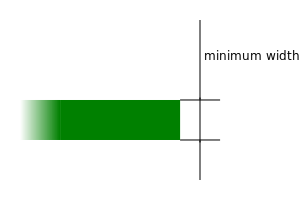
\includegraphics[height=56.4444458242mm, width=84.6666687363mm]{FIG/technology_rule_width.svg.pdf}}
  \put(204.0,-60.0){\makebox(0,0)[l]{\smash{minimum width}}}
\end{picture}
	\caption{minimum width rule}
	\label{fig:technology_rule_width}
\end{figure}

The minimum enclosure rules describe minimum distances, which need to be met between shapes on different layers. In most cases a technology file contains only minimum enclosure rules, where one of the considered layers is a via-layer. A via-layer is an additional layer during manufacturing, in which the connections between the different layers are created. For the routing these rules result in the dimensions of the vias on the layers, which they connect.

For some Via-Definitions, for example in the Hit-Kit of AMS, some enclosure rules are missing, at least in the technology file, but for the design rule check these rules are still existing. In these cases, I have to assume that there is a certain default value for the minimum enclosure rules: 0.2$\mu$m to the layer below and 0.15$\mu$m to the layer above a via-layer. These values work at least for the technology definition of AMS, but they may differ in the definition of other manufacturers.

Every via-definition must have two minimum enclosure rules, one for every layer, which is connected through the via. Additionally, we need one minimum width rule for the via-layer, which describes the width of the actual connection. From these three rules we then can calculate the dimensions of the via, which typically differ for the two layers \nref{fig:technology_rule_via_dimensions}.

\begin{equation}
\label{eq:via_dimension}
{via dimension} = 2 \cdot \text{minimum enclosure} + \text{minimum via width}
\end{equation}

\begin{figure}
	\centering
	\setlength{\unitlength}{0.282222229121mm}
\begin{picture}(360.0, 260.0)(0, -260.0)
  \put(0,-260.0){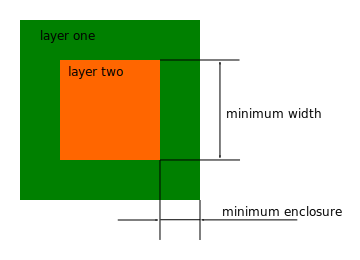
\includegraphics[height=73.3777795715mm, width=101.600002484mm]{FIG/technology_rule_via_dimensions.svg.pdf}}
  \put(226.0,-118.0){\makebox(0,0)[l]{\smash{minimum width}}}
  \put(68.0,-76.0){\makebox(0,0)[l]{\smash{layer two}}}
  \put(40.0,-40.0){\makebox(0,0)[l]{\smash{layer one}}}
  \put(222.0,-216.00002){\makebox(0,0)[l]{\smash{minimum enclosure}}}
\end{picture}
	\caption{minimum width rule}
	\label{fig:technology_rule_via_dimensions}
\end{figure}

Last but not least, there are several minimum notch rule definitions available in the technology definition of AMS. They are mostly used for the internal layout design of, for example, a transistor. During the routing they define, for instance, a minimum distance between two vias, connected by a route, as this construction forms a notch \nref{fig:technology_rule_notch}.

\begin{figure}
	\centering
	\setlength{\unitlength}{0.282222229121mm}
\begin{picture}(400.0, 180.0)(0, -180.0)
  \put(0,-180.0){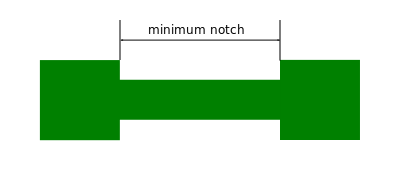
\includegraphics[height=50.8000012418mm, width=112.888891648mm]{FIG/technology_rule_notch.svg.pdf}}
  \put(148.0,-34.0){\makebox(0,0)[l]{\smash{minimum notch}}}
\end{picture}
	\caption{minimum notch between two vias}
	\label{fig:technology_rule_notch}
\end{figure}

\section{Electrical Rules}
\label{sec:electrical_rules}
In the tech-file from the manufacturer there also are electrical rules implied. These rules describe the exact electrical behaviour and can be used, for example, for a simulation of the whole circuit. In the routing algorithms, that will be described later on \nref{sec:implemented_algorithms} I will use these values to optimize the behaviour of the circuit layout. Therefore, I want to describe how they can be interpreted.

The first important value is the sheet resistance. This value defines the resistance of a layer and I use it to calculate the resistance of the routes. I do not need an exact resistance, only a tool to measure and compare, which takes the different layers into account. Therefore, my personal definition for this algorithm of the sheet resistance will possibly be not the right one. But in my point of view it is useful in this case. For routes on one layer I just multiply the sheet resistance value with the length of the route, as I always use the minimum width for routes. A via doesn't really have a length, so I multiply the value with the area. Afterwards, these two results are summed up for a whole connection and this then represents the resistance of this connection.

The other two used values are the edge- and area-capacitance. The edge-capacitance illustrates the capacity between two neighbour routes on the same layer, whereas the area-capacitance describes the capacity between two routes on the same position but on different layers. The total capacities ($C_e$ and $C_a$) are calculated from the length where two routes are neighbours ($l$), the distance between them ($d$) in case of an edge capacitor, the width they overlap, ($w$) in case of an area capacity, and the values from the technology file ($C'_e$ and $C'_a$).
\[C_a = C'_a \cdot l \cdot w\]
\[C_e = C'_e \cdot \frac{l}{d}\]

All in all, the aforementioned definitions are most likely not the right ones but the results are multiplied with adjustable weights afterwards anyway. Therefore, the exact values are not a matter of interest, the results are only used as rough estimations and measurement.





